% ========================================
%	Header einbinden
% ========================================

\documentclass[bibtotoc,titlepage]{scrartcl}

% Deutsche Spracheinstellungen
\usepackage[ngerman,german]{babel, varioref}
\usepackage[T1]{fontenc}
\usepackage[utf8]{inputenc}

%\usepackage{marvosym}

\usepackage{amsfonts}
\usepackage{amssymb}
\usepackage{amsmath}
\usepackage{amscd}
\usepackage{amstext}

\usepackage{longtable}

%\usepackage{bibgerm}

\usepackage{footnpag}

\usepackage{ifthen}                 %%% package for conditionals in TeX
\usepackage[amssymb]{SIunits}
%Für textumflossene Bilder und Tablellen
%\usepackage{floatflt} - veraltet

%Für Testzwecke aktivieren, zeigt labels und refs im Text an.
%\usepackage{showkeys}

% Abstand zwischen zwei Absätzen nach DIN (1,5 Zeilen)
% \setlength{\parskip}{1.5ex plus0.5ex minus0.5ex}

% Einrückung am Anfang eines neuen Absatzes nach DIN (keine)
%\setlength{\parindent}{0pt}

% Ränder definieren
% \setlength{\oddsidemargin}{0.3cm}
% \setlength{\textwidth}{15.6cm}

% bessere Bildunterschriften
%\usepackage[center]{caption2}


% Problemlösungen beim Umgang mit Gleitumgebungen
\usepackage{float}

% Nummeriert bis zur Strukturstufe 3 (also <section>, <subsection> und <subsubsection>)
%\setcounter{secnumdepth}{3}

% Führt das Inhaltsverzeichnis bis zur Strukturstufe 3
%\setcounter{tocdepth}{3}
\usepackage[version=3]{mhchem}
	\mhchemoptions{minus-sidebearing-left=0.06em, minus-sidebearing-right=0.11em}
\usepackage{exscale}

\newenvironment{dsm} {\begin{displaymath}} {\end{displaymath}}
\newenvironment{vars} {\begin{center}\scriptsize} {\normalsize \end{center}}


\newcommand {\en} {\varepsilon_0}               % Epsilon-Null aus der Elektrodynamik
\newcommand {\lap} {\; \mathbf{\Delta}}         % Laplace-Operator
\newcommand {\R} { \mathbb{R} }                 % Menge der reellen Zahlen
\newcommand {\e} { \ \mathbf{e} }               % Eulersche Zahl
\renewcommand {\i} { \mathbf{i} }               % komplexe Zahl i
\newcommand {\N} { \mathbb{N} }                 % Menge der nat. Zahlen
\newcommand {\C} { \mathbb{C} }                 % Menge der kompl. Zahlen
\newcommand {\Z} { \mathbb{Z} }                 % Menge der kompl. Zahlen
\newcommand {\limi}[1]{\lim_{#1 \rightarrow \infty}} % Limes unendlich
\newcommand {\sumi}[1]{\sum_{#1=0}^\infty}
\newcommand {\rot} {\; \mathrm{rot} \,}         % Rotation
\newcommand {\grad} {\; \mathrm{grad} \,}       % Gradient
\newcommand {\dive} {\; \mathrm{div} \,}        % Divergenz
\newcommand {\dx} {\; \mathrm{d} }              % Differential d
\newcommand {\cotanh} {\; \mathrm{cotanh} \,}   %Cotangenshyperbolicus
\newcommand {\asinh} {\; \mathrm{areasinh} \,}  %Area-Sinus-Hyp.
\newcommand {\acosh} {\; \mathrm{areacosh} \,}  %Area-Cosinus-H.
\newcommand {\atanh} {\; \mathrm{areatanh} \,}  %Area Tangens-H.
\newcommand {\acoth} {\; \mathrm{areacoth} \,}  % Area-cotangens
\newcommand {\Sp} {\; \mathrm{Sp} \,}
\newcommand {\mbe} {\stackrel{\text{!}}{=}}     %Must Be Equal
\newcommand{\qed} { \hfill $\square$\\}
\renewcommand{\i} {\imath}
\def\captionsngerman{\def\figurename{\textbf{Abb.}}}

%%%%%%%%%%%%%%%%%%%%%%%%%%%%%%%%%%%%%%%%%%%%%%%%%%%%%%%%%%%%%%%%%%%%%%%%%%%%
% SWITCH FOR PDFLATEX or LATEX
%%%%%%%%%%%%%%%%%%%%%%%%%%%%%%%%%%%%%%%%%%%%%%%%%%%%%%%%%%%%%%%%%%%%%%%%%%%%
%%%
\ifx\pdfoutput\undefined %%%%%%%%%%%%%%%%%%%%%%%%%%%%%%%%%%%%%%%%% LATEX %%%
%%%
\usepackage[dvips]{graphicx}       %%% graphics for dvips
\DeclareGraphicsExtensions{.eps,.ps}   %%% standard extension for included graphics
\usepackage[ps2pdf]{thumbpdf}      %%% thumbnails for ps2pdf
\usepackage[ps2pdf,                %%% hyper-references for ps2pdf
bookmarks=true,%                   %%% generate bookmarks ...
bookmarksnumbered=true,%           %%% ... with numbers
hypertexnames=false,%              %%% needed for correct links to figures !!!
breaklinks=true,%                  %%% breaks lines, but links are very small
linkbordercolor={0 0 1},%          %%% blue frames around links
pdfborder={0 0 112.0}]{hyperref}%  %%% border-width of frames
%                                      will be multiplied with 0.009 by ps2pdf
%
\hypersetup{ pdfauthor   = {Hannes Franke; Julius Tilly},
pdftitle    = {V301 Innenwiderstand und Leistungsanpassung}, pdfsubject  = {Protokoll FP}, pdfkeywords = {V301, Innenwiderstand, Leistungsanpassung},
pdfcreator  = {LaTeX with hyperref package}, pdfproducer = {dvips
+ ps2pdf} }
%%%
\else %%%%%%%%%%%%%%%%%%%%%%%%%%%%%%%%%%%%%%%%%%%%%%%%%%%%%%%%%% PDFLATEX %%%
%%%
\usepackage[pdftex]{graphicx}      %%% graphics for pdfLaTeX
\DeclareGraphicsExtensions{.pdf}   %%% standard extension for included graphics
\usepackage[pdftex]{thumbpdf}      %%% thumbnails for pdflatex
\usepackage[pdftex,                %%% hyper-references for pdflatex
bookmarks=true,%                   %%% generate bookmarks ...
bookmarksnumbered=true,%           %%% ... with numbers
hypertexnames=false,%              %%% needed for correct links to figures !!!
breaklinks=true,%                  %%% break links if exceeding a single line
linkbordercolor={0 0 1},
linktocpage]{hyperref} %%% blue frames around links
%                                  %%% pdfborder={0 0 1} is the default
\hypersetup{
pdftitle    = {V301 Innenwiderstand und Leistungsanpassung}, 
pdfsubject  = {Protokoll AP}, 
pdfkeywords = {V301, Innenwiderstand, Leistungsanpassung},
pdfsubject  = {Protokoll AP},
pdfkeywords = {V301, Innenwiderstand, Leistungsanpassung}}
%                                  %%% pdfcreator, pdfproducer,
%                                      and CreationDate are automatically set
%                                      by pdflatex !!!
\pdfadjustspacing=1                %%% force LaTeX-like character spacing
\usepackage{epstopdf}
%
\fi %%%%%%%%%%%%%%%%%%%%%%%%%%%%%%%%%%%%%%%%%%%%%%%%%%% END OF CONDITION %%%
%%%%%%%%%%%%%%%%%%%%%%%%%%%%%%%%%%%%%%%%%%%%%%%%%%%%%%%%%%%%%%%%%%%%%%%%%%%%
% seitliche Tabellen und Abbildungen
%\usepackage{rotating}
\usepackage{ae}
\usepackage{
  array,
  booktabs,
  dcolumn
}
\makeatletter 
  \renewenvironment{figure}[1][] {% 
    \ifthenelse{\equal{#1}{}}{% 
      \@float{figure} 
    }{% 
      \@float{figure}[#1]% 
    }% 
    \centering 
  }{% 
    \end@float 
  } 
  \makeatother 


  \makeatletter 
  \renewenvironment{table}[1][] {% 
    \ifthenelse{\equal{#1}{}}{% 
      \@float{table} 
    }{% 
      \@float{table}[#1]% 
    }% 
    \centering 
  }{% 
    \end@float 
  } 
  \makeatother 
%\usepackage{listings}
%\lstloadlanguages{[Visual]Basic}
%\allowdisplaybreaks[1]
%\usepackage{hycap}
%\usepackage{fancyunits}

\usepackage{textcomp}
\usepackage{caption}
\usepackage{float}


\newfloat{formel}{H}{for}
\floatname{formel}{Formel}

% ========================================
%	Angaben für das Titelblatt
% ========================================

\title{Versuch\\602 - Röntgen-Emissions- und Absorbtionsspektren				% Titel des Versuchs 
\large TU Dortmund, Fakultät Physik\\ 
\normalsize Anfänger-Praktikum}

\author{Jan Adam\\			% Name Praktikumspartner A
{\small \href{jan.adam@tu-dortmund.de}{jan.adam@tu-dortmund.de}}	% Erzeugt interaktiven einen Link
\and						% um einen weiteren Author hinzuzfügen
Dimitrios Skodras\\					% Name Praktikumspartner B
{\small \href{dimitrios.skodras@tu-dortmund.de}{dimitrios.skodras@tu-dortmund.de}}		% Erzeugt interaktiven einen Link
}
\date{13.November 2012}				% Das Datum der Versuchsdurchführung

% ========================================
%	Das Dokument beginnt
% ========================================

\begin{document}

% ========================================
%	Titelblatt erzeugen
% ========================================

\maketitle					% Jetzt wird die Titelseite erzeugt
\thispagestyle{empty} 				% Weder Kopfzeile noch Fußzeile

% ========================================
%	Der Vorspann
% ========================================

%\newpage					% Wenn Verzeichnisse auf einer neuen Seite beginnen sollen
%\pagestyle{empty}				% Weder Kopf- noch Fußzeile für Verzeichnisse

\tableofcontents

%\newpage					% eine neue Seite
%\thispagestyle{empty}				% Weder Kopf- noch Fußzeile für Verzeichnisse
%\listoffigures					% Abbildungsverzeichnis

%\newpage					% eine neue Seite
%\thispagestyle{empty}				% Weder Kopf- noch Fußzeile für Verzeichnisse
%\listoftables					% Tabellenverzeichnis
\newpage					% eine neue Seite


% ========================================
%	Kapitel
% ========================================

\section{Einleitung}				% Bei Bedarf
Wilhelm Conrad Röntgen (\textborn 1845 in Remscheid; \textdied 1923 in München), entdeckte 1895 in der 
Julius-Maximilians-Universität Würzburg die nach ihm benannten Röntgenstrahlen, von ihm selbst und im 
englisch-sprachigen Raum auch X-Strahlen (engl. \textit{X-Rays}) genannt. In diesem Versuch geht es um
die Untersuchung des Emissionsspektrums der Röntgenstrahlung, sowie der Absorbtionsspektren verschieden schwerer
Elemente.
\section{Theorie}
\subsection{Das Emissionsspektrum}
Die erforderlichen Röntgenstrahlen entstehen durch schnelle Elektronen. Hierbei werden aus einer Glühkathode freie Elektronen
thermisch emittiert, woraufhin sie in einem evakuierten Glaskolben mittels einer Anode mit einer Spannung $U_b$ mehrerer kV beschleunigt werden. Dort prallen sie
auf und durch im Folgenden aufgeführte Prozesse entsteht Röntgenstrahlung.

\begin{figure}[H]
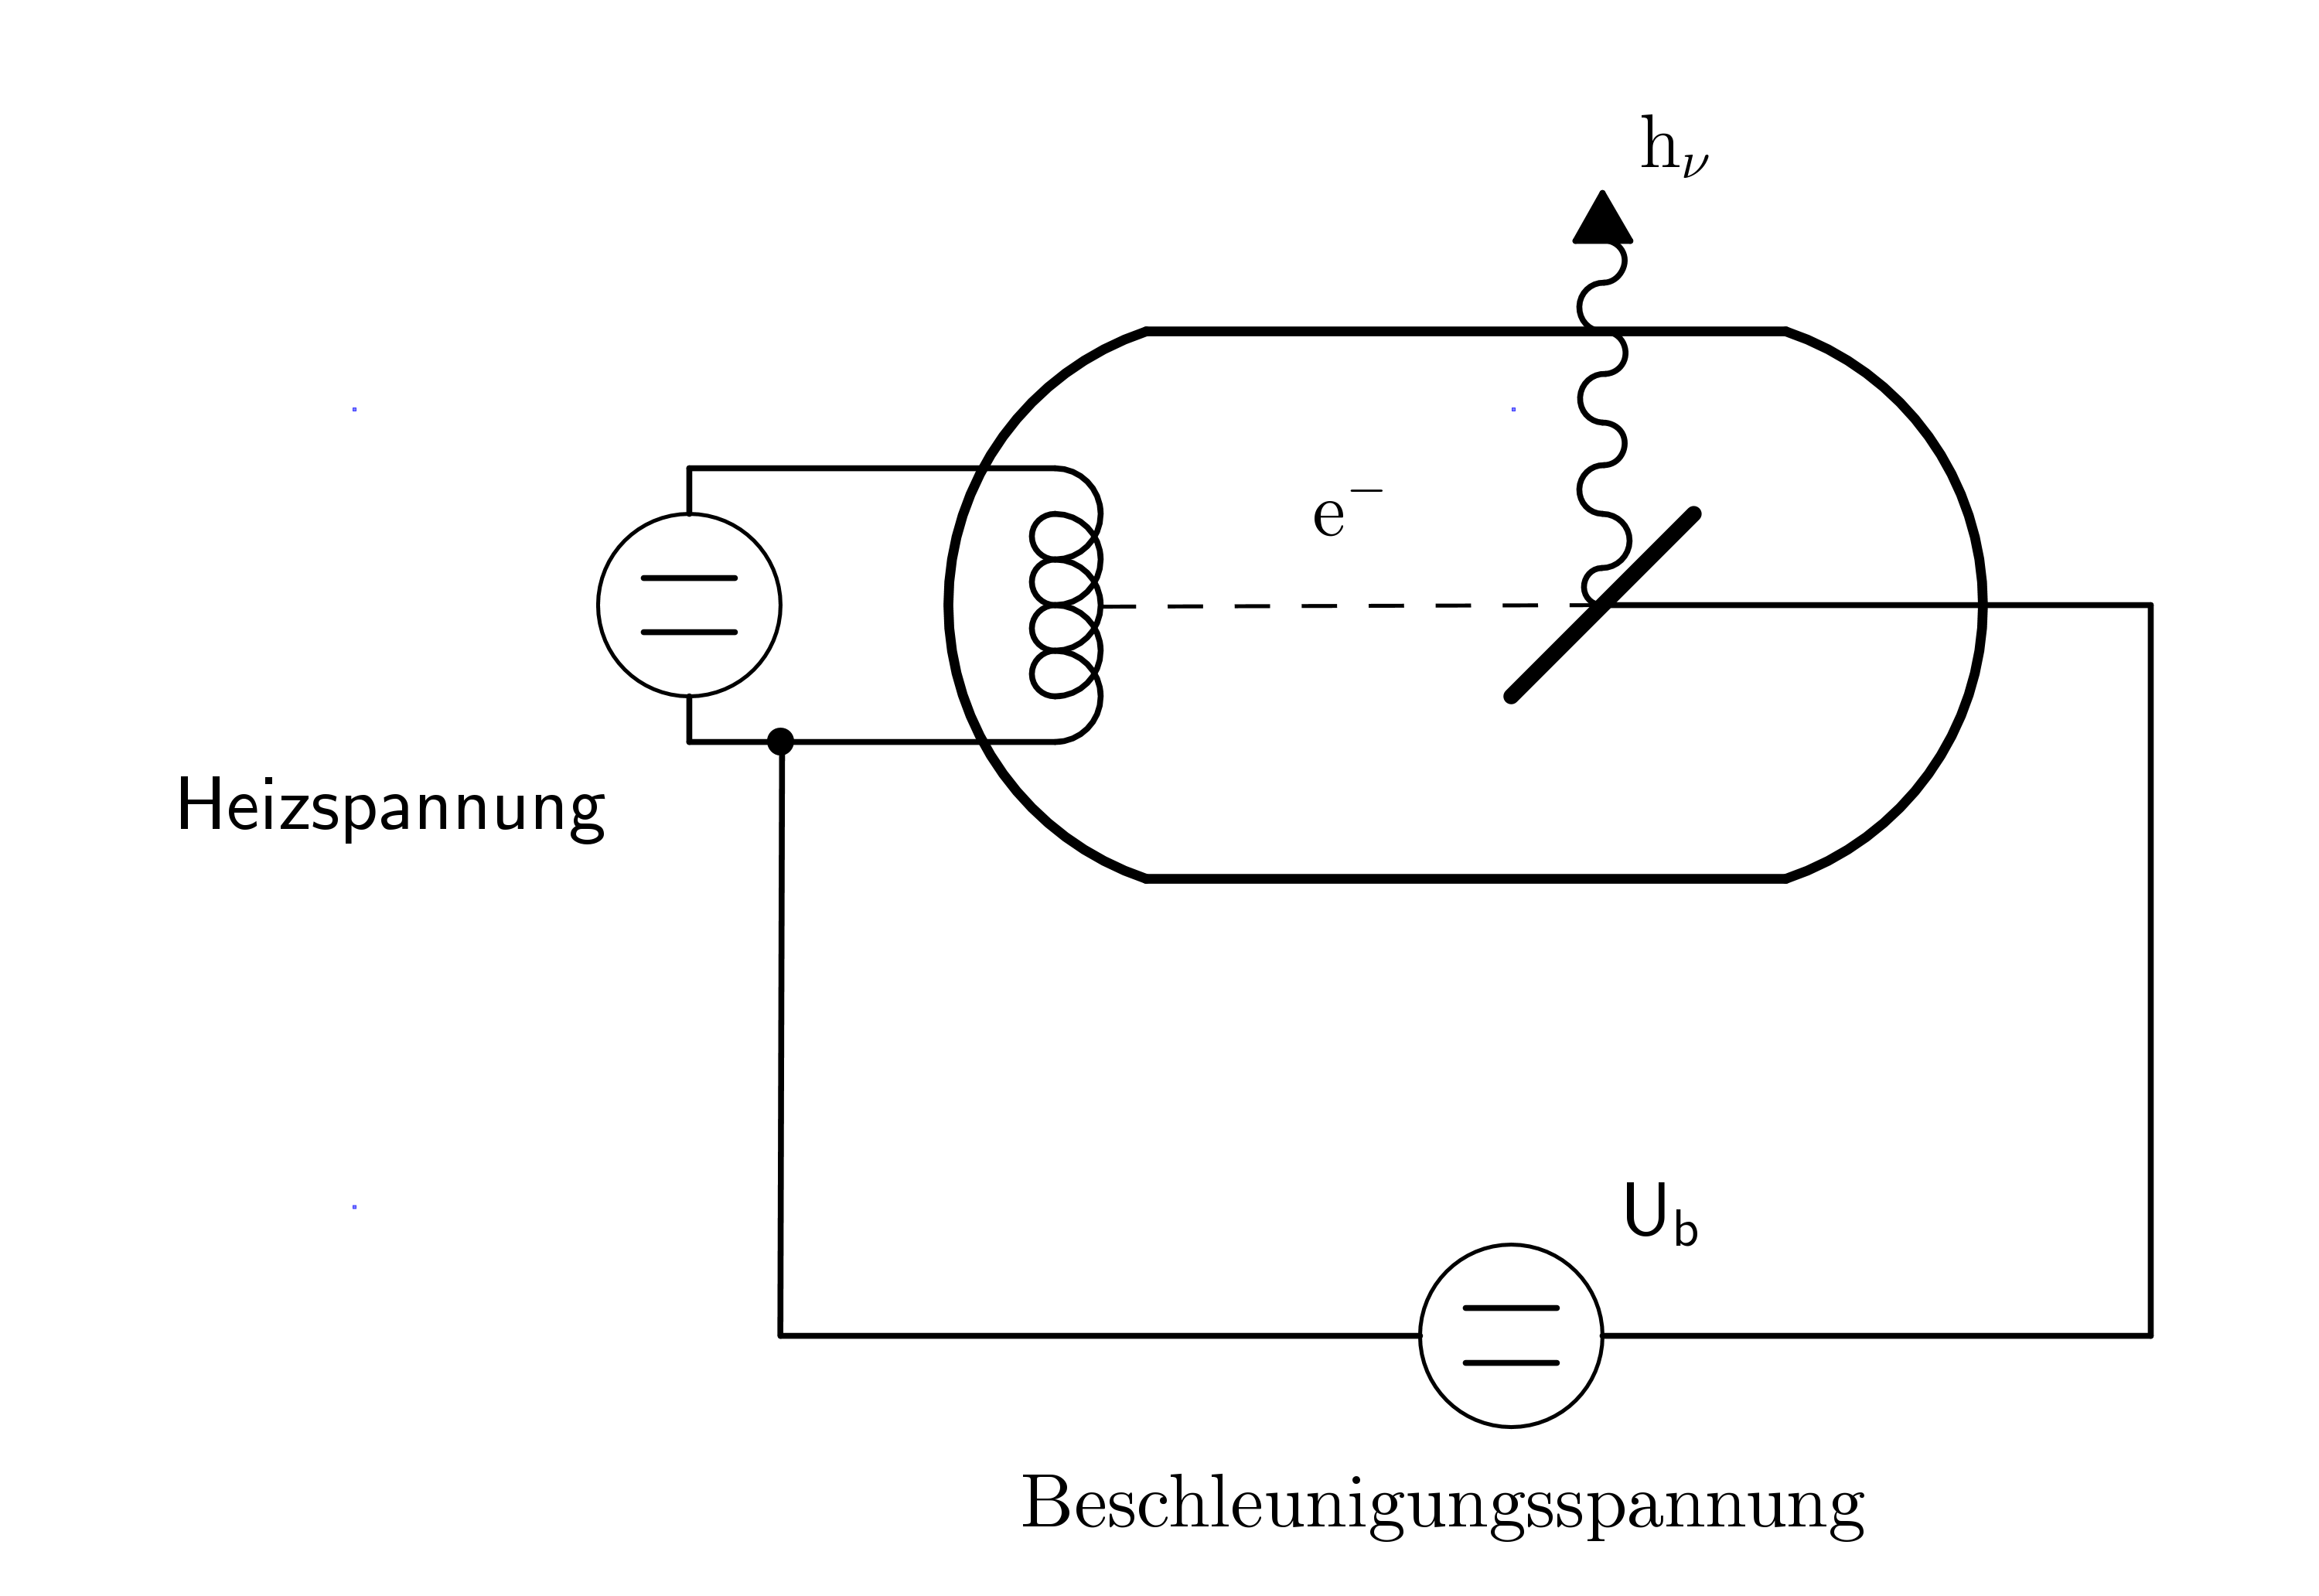
\includegraphics[width=0.7\textwidth] {pics/602a.png}
\centering
\caption{Schematischer Aufbau einer Röntgenröhre}
\end{figure}
\subsubsection[Arten von Röntgenstrahlen]{Bremsstrahlung und charakteristische Röntgenstrahlung}
\label{BcR}

Mit einer geringen Wahrscheinlichkeit können die schnellen Elektronen tiefer in die Atome des Anodenmaterials eintreten und
damit in das Coulombpotenzial des Kerns. Durch die dort wirkenden elektromagnetischen Kräfte erfahren die freien Elektronen
eine Änderung ihrer geradlinigen Bewegung und damit eine Beschleunigung. Beschleunigte Ladungsträger emittieren bekannterweise
Photonen, deren Energiebereich kontinuierlich von quasi Null einem Maximalwert begrenzt wird, welcher der anfänglichen kinetischen Energie
des Elektrons gleicht. Die so entstehende Strahlung wird Bremsstrahlung genannt.\\
Statt das Atom nur zu passieren, wechselwirkt die charakteristische Röntgenstrahlung mit den Elektronen innerer Schalen. In einem
Atom sind die Elektronen durch die Coulombkraft an den Kern mit einer gewissen eindeutigen Energie gebunden. Wenn nun ein schnelles
freies Elektron hinreichend viel kinetische Energie hat, ist es in der Lage, ein Elektron der inneren Schalen zu stoßen und
aus dem Atom zu schleudern. Das ionisierte Atom reagiert mit kaskadenartigem Nachrücken von Elektronen äußer Schalen. Wie zuvor gesagt,
besitzen Elektronen eine eindeutige Bindungsenergie zum Kern, was bedeutet, dass der Übergang zwischen den Schalen mit diskreten
Energiedifferenzen verbunden ist. Diese Differenzen führen zur Entstehung von Photonen im Energiebereich der Röntgenstrahlung.

\begin{figure}[H]
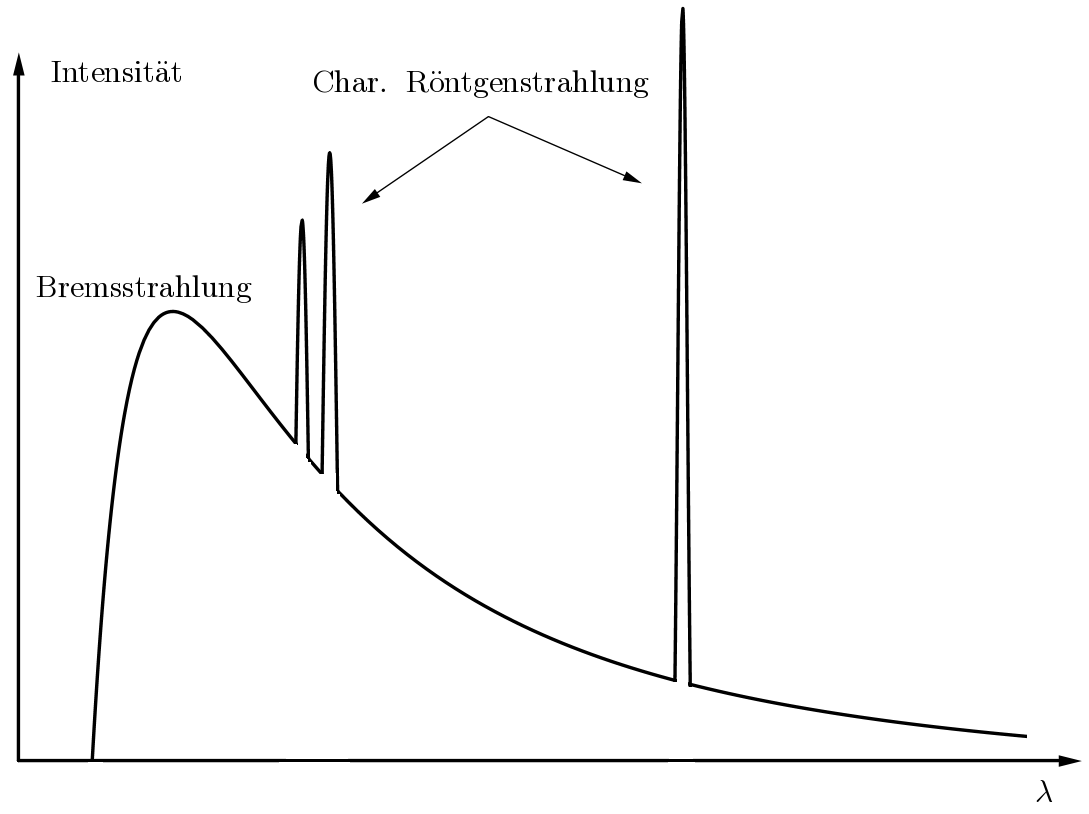
\includegraphics[width=0.7\textwidth] {pics/602b.png}
\centering
\caption{Intensitätsverteilung der Röntgenstrahlen in Abhängigkeit der Wellenlänge}
\label{602b}
\end{figure}

Da die kinetische Energie der Elektronen durch die Beschleunigungsspannung festgelegt ist, wird die kürzeste Wellenlänge eines 
Photons wie folgt ausgedrückt:

\begin{formel}
\begin{equation}
 E_{Ph} = h \cdot \frac{c}{\lambda} = e_0 \cdot U_b = E_{kin} \Leftrightarrow \lambda_{min} = \frac{h \cdot c}{e_0 \cdot U}
 \end{equation}
 \caption*{\small{(h = Plancksches Wirkungsquantum, $e_0$ = Elementarladung, c = Lichtgeschwindigkeit)}}
\end{formel}
 
\subsubsection[Die Grobstruktur]{Grobstruktur des Emissionsspektrums}
\label{grob}
Da die Röntgenemission ein Vielteilchenproblem ist, wird um an die Energieeigenwerte heranzukommen, eine Einelektronenanregung
betrachtet. Hierbei wird der Einfluss des Kerns sowie der anderen Elektronen auf ein beteiligtes Elektron hergenommen und durch
eine effektive Größe $z_{eff}$ ausgedrückt, statt durch die Kernladungszahl $z$. Unter dieser Voraussetzung wird gemäß der Schrödinger-Gleichung
bei einem Elektronenübergang von der m-ten zur n-ten Schale folgende Energie frei:

\begin{formel}
\begin{equation}
  h\cdot\nu_{m,n} = R_{\infty}  z_{eff_{m,n}}^2 \cdot \left( \frac{1}{n^2} - \frac{1}{m^2} \right)
\end{equation}
\caption*{\small{(R = Rydbergkonstante, n,m = Hauptquantenzahlen)}}
\label{Emn}
\end{formel}

Die innerste Schale (n=1) wird hierbei als K-Schale bezeichnet und alphabetisch fortschreitend für größere n. Wie in Abbildung \eqref{Niveaus}
zu sehen ist, dass die L-Serie, also alle Übergänge auf das L-Niveau, energetisch niedriger sind, als die K-Serie, was an der
1/n-Abhängigkeit liegt. Anhand der Energie bei Übergängen für kleine n und m erkennt man deutliche Unterschiede zu jene für große
n und m. So entsteht Röntgenstrahlung auch nur, wenn Wechselwirkungen mit den innersten Schalen vorkommen.

\begin{figure}[H]
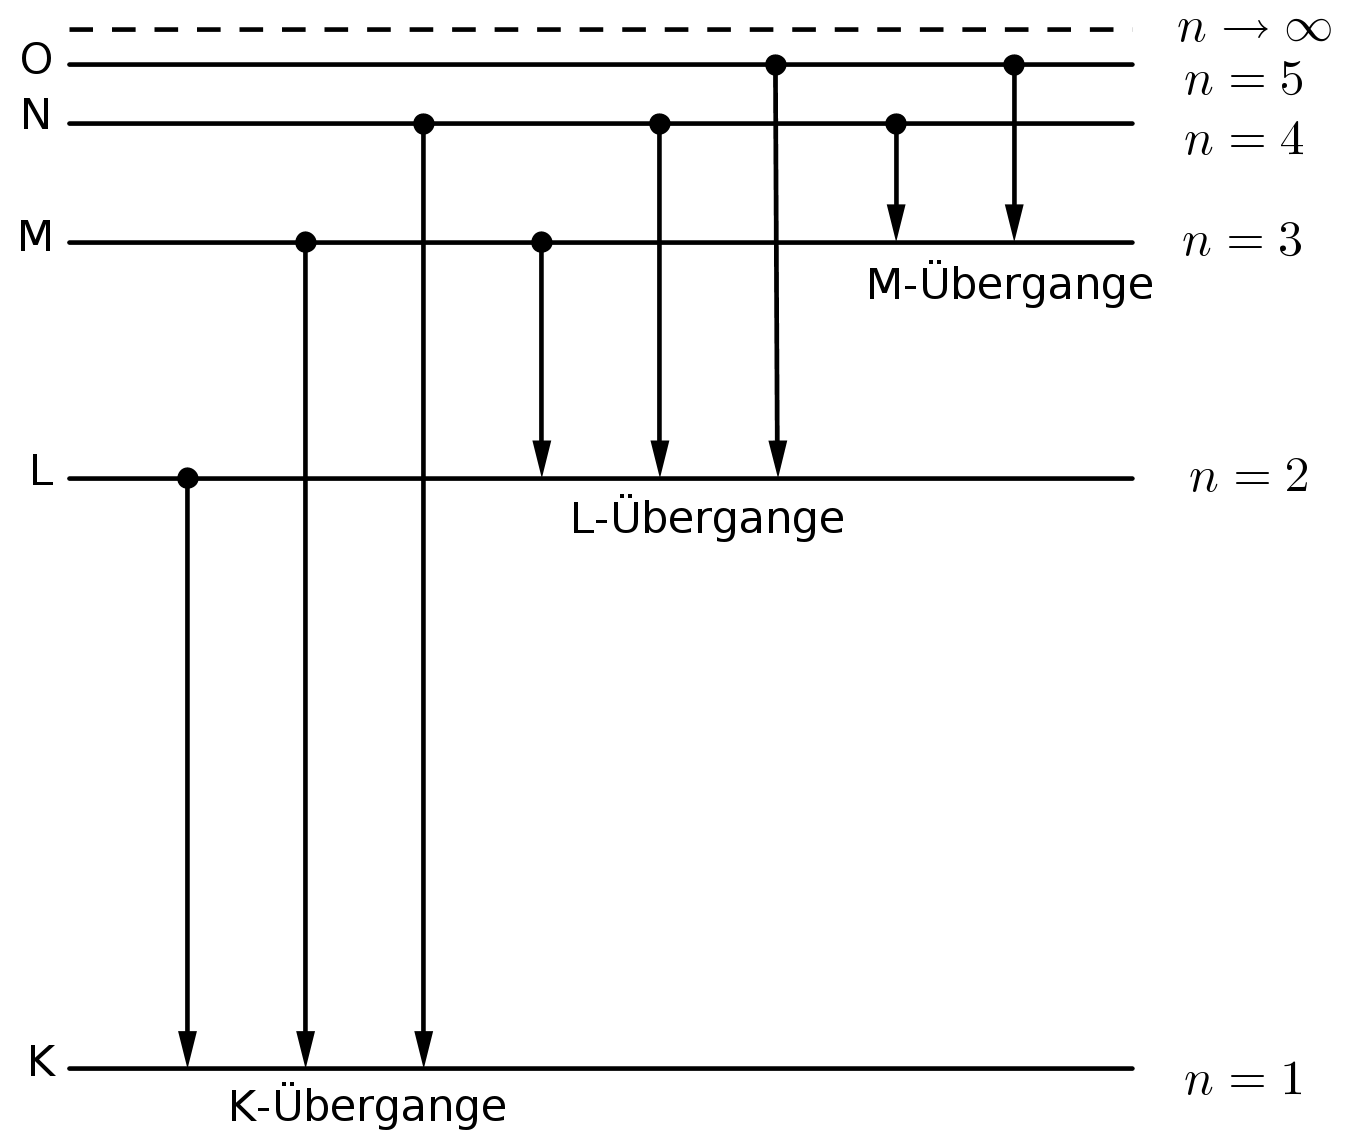
\includegraphics[width=0.7\textwidth] {pics/602c.png}
\centering
\caption{Mögliche Röntgenübergänge in einer Elektronenhülle}
\label{Niveaus}
\end{figure}

\subsubsection[Die Feinstruktur]{Feinstruktur des Emissionsspektrums}
Anders als Gleichung (2) bietet im Rahmen der Störungsrechnung die Sommerfeldsche Feinstrukturformel eine bessere Näherung
für m $\rightarrow \infty$.

\begin{formel}
\begin{equation}
  h\cdot\nu_{n,j} = -R_{\infty}  \left\{ z_{eff_{1}}^2 \cdot \frac{1}{n^2} + \alpha^2 z_{eff_{2}}^4 \cdot \frac{1}{n^3} \left( \frac{1}{j+\frac12}-\frac{3}{4n}\right)\right\}
  \label{Enj}
\end{equation}
\caption*{\small{($\alpha$ = Sommerfeldsche Feinstrukturkonstante, j = Gesamtdrehimpulszahl)}}
\end{formel}

wobei sich j und $z_{eff_{1,2}}$ folgendermaßen ergeben:

\begin{equation*}
 j = l \pm \frac12, \qquad z_{eff_{1}} = z - \sigma, \qquad z_{eff_{2}} = z - s
\end{equation*}

Hierbei ist l die Bahndrehimpulsquantenzahl und $\sigma$ und s sogenannte Abschirmungszahlen. Die Konstante der vollständigen
Abschirmung $\sigma$ wird im Wesentlichen durch die Hüllenelektronen bestimmt, deren Ladungsverteilung in der n-ten Schale
ihr Maximum erreicht, sowie durch die äußeren Elektronen. s, als Konstante der inneren Abschirmung, wird nur durch die Elektronen
der n-ten Schale bestimmt. Andere Einflüsse der Kernladung sind nicht feststellbar.


\begin{figure}[H]
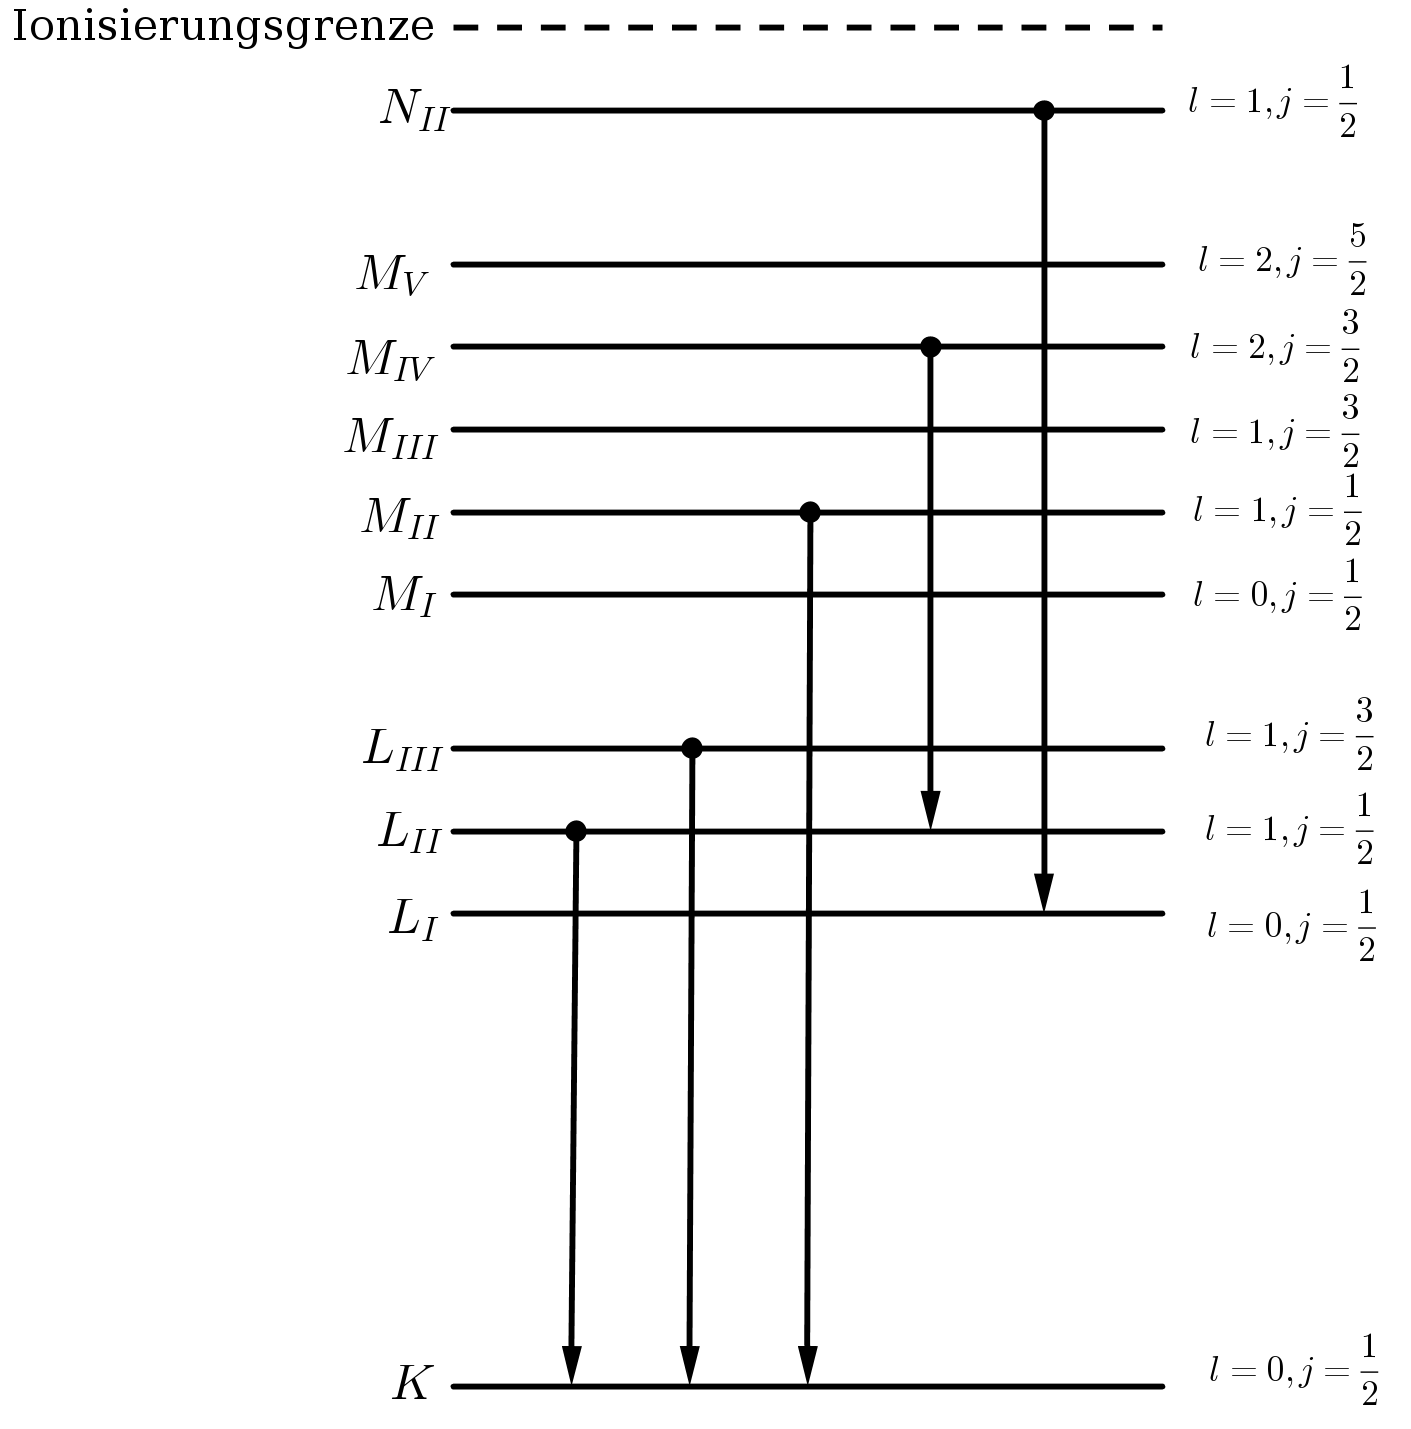
\includegraphics[height=0.56\textheight] {pics/602d.png}
\centering
\caption{Feinstruktur-Aufspaltung}
\label{FS}
\end{figure}


Da es neben n nun auch mehrere l- und j-Werte gibt, kann man die in \ref{grob} genannten Niveaus noch unterteilen, auch 
Feinstruktur-Aufspaltung genannt. Mit der Überlegung, dass $l_{max} = n-1$ ist, ergeben sich die in Abbildung \eqref{FS}
veranschaulichten Feinstrukturniveaus. Da für die K-Schale mit n=1 l=0 ist, haben die Elektronen dort keinen Bahndrehimpuls
und damit gibt es hier keine Substruktur. Für die L-Schale sind l=0 und l=1 denkbar. Daher ergibt sich für die Drehimpulszahlen
zu $[l=1,j=\frac32]$, $[l=1,j=\frac12],[l=0,j=\frac12] $. Also drei Unterniveaus.\\
Bei den Übergängen sind nicht alle Kombinationen möglich. Für das Wechseln des Energieniveaus gibt es folgende zwei Einschränkungen.
Zum einen darf die Änderung des Bahndrehimpuls zweier beteiligter Niveaus nur $\Delta l = \pm1$ betragen. Zum anderen werden
alle Übergänge für $\Delta n \ge 3$ als sehr unwahrscheinlich angesehen.

\subsection{Das Absorbtionsspektrum}
Die Intensität der Röntgenstrahlen nimmt beim Passieren von Materie energie- und materialabhängig ab. Im Wesentlichen 
ist das auf Absorbtion zurückzuführen. Geringfügig auch auf Streuung.
\subsubsection{Innerer Photo-Effekt}
Diese Absorbtion wird innerer Photo-Effekt genannt. Hierbei dringt ein hoch energetisches Photon in die inneren Schalen
des Atoms vor, im Gegensatz zum äußeren Photo-Effekt, und überträgt einem Elektron seine Energie. Da die umliegenden Schalen
allesamt besetzt sind, ist eben dieser Energiebetrag erforderlich, um das gestoßene Elektron aus dem Atom mit einer endlichen
kinetischen Restenergie zu befördern. Daher muss dieser Lichtquant auch mindestens diese Energie aufbringen. Speziell für die
K-Schale gilt daher nach \eqref{Enj}:

\begin{equation}
 h\nu_{K_{Abs}} = E_{1,\frac12} - E_{\infty} = R_{\infty}\left\{(z-\sigma_{1,0})^2 + \alpha^2(z - s_{1,0})^4\cdot \frac14\right\}
 \label{K1}
\end{equation}

$s_{1,0}$ verschwindet für wenige Elektronen, was auf der K-Schale für zwei Elektronen gegeben ist. So lässt sich nun $\sigma_{1,0}$
durch eine Messung von $h\nu_{K_{Abs}}$ bestimmen. Die drei L-Absorbtionsenergien lassen sich als weiteres Beispiel wie folgt 
aus \eqref{Enj} ermitteln:

\begin{align}
  h\nu_{L_{Abs,I}} &= E_{2,0,\frac12} - E_{\infty} = R_{\infty}\left\{\frac{(z-\sigma_{2,0})^2}{8} + \alpha^2\frac{(z - s_{2,0})^4}{8}\cdot \frac58\right\}, 
  \label{L1} \\
  h\nu_{L_{Abs,II}} &= E_{2,1,\frac12} - E_{\infty} = R_{\infty}\left\{\frac{(z-\sigma_{2,1})^2}{4} + \alpha^2\frac{(z - s_{2,1})^4}{8}\cdot \frac58\right\},
 \label{L2}\intertext{sowie}
  h\nu_{L_{Abs,III}} &= E_{2,1,\frac32} - E_{\infty} = R_{\infty}\left\{\frac{(z-\sigma_{2,1})^2}{4} + \alpha^2\frac{(z - s_{1,0})^4}{8}\cdot \frac18\right\}.
 \label{L3}
\end{align}

$s_{2,1}$ lässt sich nun über die Differenz von \eqref{L2} und \eqref{L3} berechnen.

\begin{equation}
 h\nu_{L_{Abs,II}} - h\nu_{L_{Abs,III}} = R_{\infty}\, \alpha^2 \frac{(z-s_{2,1})^4}{16}
\end{equation}

\subsubsection{Fluoreszens-Strahlung und Compton-Effekt}
Weitere Effekte, die bei der Wechselwirkung von Röntgenstrahlung und Materie auftreten sind die Floureszens-Strahlung und 
der Compton-Effekt. Ähnlich wie bei der charakteristischen Röntgenstrahlung unter \ref{BcR} auf Seite \pageref{BcR} entstehen
durch das Emittieren eines inneren Elektrons kaskadenartige Elektronenübergänge äußerer Schalen auf innere. Hierbei wird ebenfalls
für das Material charakteristische Röntgenstrahlung frei. Im Gegensatz zum Photo-Effekt ionsiert ein Photon nicht das Atom,
sondern gibt lediglich einen Teil seiner Energie und seines Impulses an ein nahezu freies Elektron ab und bewegt sich danach
mit verringertem Energie- und Impulswert in geänderter Richtung fort. Das erklärt die Abnahme der Intensität in diesen 
Energiebereichen (Compton-Kontinuum).

\subsection{Messung von Intensität und Energie der Röntgenstrahlung}
Die in \eqref{K1},  \eqref{L1},  \eqref{L2}  und \eqref{L3} aufgeführten Absorbtionsenergien müssen nun auch experimentell
bestimmt werden. Hierzu wird eine Probe des betrachteten Materials mit geringer Dicke mit monoenergetischen Röntgenquanten
bestrahlt und die Intensität, also die Messungen pro Zeit und Fläche, in Abhängigkeit der Energie aufgetragen. 
Wenn die Energie ausreicht, werden Elektronen innerer Schalen herausgestoßen und die Intensitätskurve erhält an dieser Stelle 
eine Unstetigkeitsstelle,die idealerweise eine Kante ergibt (Abbildung \eqref{602b}), daher auch Absorbtionskante. Wegen
der ionisierenden Wirkung der Röntgenstrahlung wird zur Intensitätsmessung häufig ein Geiger-Müller-Zählrohr in
Verbindung mit einem elektronischen Zählwerk genutzt. Mit aufwendigeren Messgeräten, wie einem Szintillations-Detektor können
auch Energiewerte der Quanten ermittelt werden, indem bei Registrierung eines Quants ein zur Quantenenergie proportionaler 
elektrischer Impuls abgegeben wird.

Für dieses Experiment wird jedoch die Welleneigenschaft der Röntgenstrahlung zur Energiewertbestimmung genutzt. Kristalle,
mit ihrer räumlich periodischen Anordnung sind geeignet, um einfallende Photonen in alle Raumrichtungen elastisch zu streuen. 
Das Interferenzmodell sagt aus, dass dann konstruktive Interferenz entsteht, wenn der Gangunderschied $\Delta$s ein 
ganzzahliges Vielfaches der Wellenlänge $\lambda$ ist.

\begin{figure}[H]
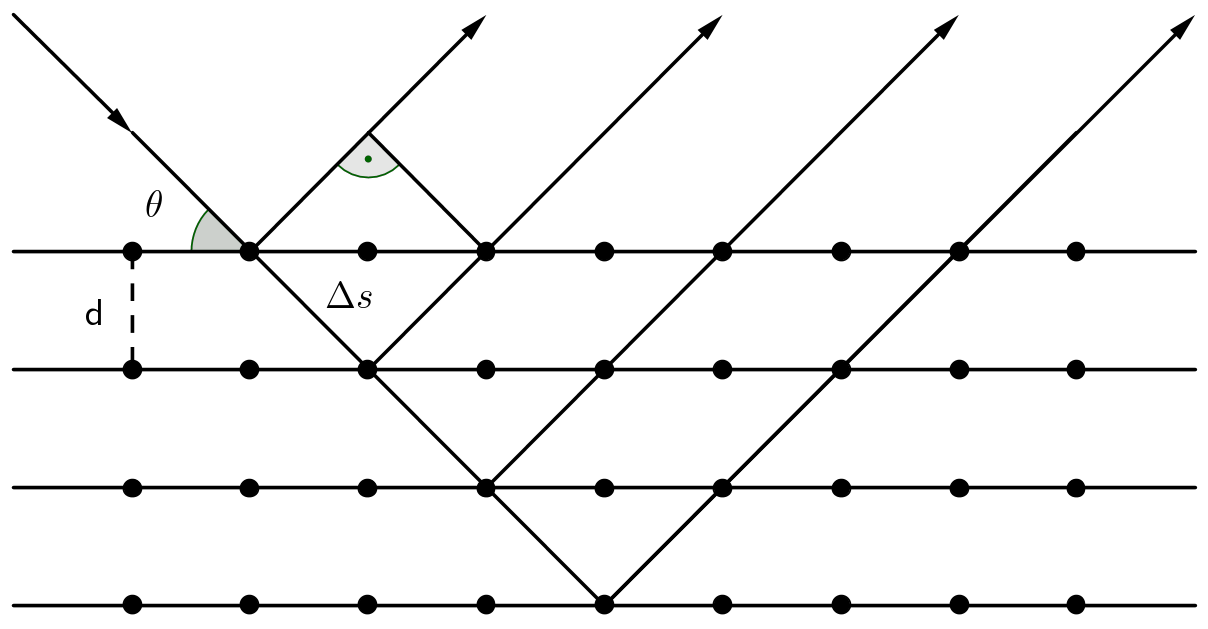
\includegraphics[width=0.8\textwidth] {pics/602e.png}
\centering
\caption{Interferenz am Kristallgitter ($\Delta s$ ist der Weg, den ein benachbarter Strahl mehr zurücklegen muss)}
\label{Gitter}
\end{figure}

Für den Gangunterschied gilt:
\begin{equation}
 \Delta s = n \cdot \lambda = 2d\sin(\theta) \qquad \text{mit} \qquad n \in \mathbb{N}.
\end{equation}

Diese Gleichung wird als Braggsche Reflexionsbedingung bezeichnet. d ist hierbei der Gitterabstand, $\theta$ ist der 
Einfallswinkel der Röntgenstrahlen und $\lambda$ ihre Wellenlänge. Die Energie der Röntgenstrahlung kann nun wie folgt
berechnet werden:

\begin{align}
E = h\nu = \frac{h c}{\lambda} = \frac{h c\cdot n}{2d\sin(\theta)}
\label{Bragg}
\end{align}

Neben dem Nutzen, eine einfache Energie-Winkel-Beziehung zu haben, kann man mit einem Kristall aus polyenergetischer
Strahlung nahezu monoenergetische erzeugen.

\section{Durchführung}
Die für die Auswertung interessanten Parameter des in Abbildung \ref{Aufbau} dargestellten Versuchsaufbaus für das Experiment
sind gegeben durch:

\renewcommand{\arraystretch}{1.5}
\begin{table}[H]
 \begin{tabular}{|c|c|}
\hline
Beschleunigungsspannung $U_b$ & 10-24 kV\\
\hline
Anodenmaterial & Kupfer ($_{29}$Cu)\\
\hline
Schwenkkristall & LiF-Einkristall\\
\hline
Netzabstand d  & 2,01 \AA \\
\hline
Interferenzordnung n & 1\\
\hline
\end{tabular}
\caption{Parameter des Versuchsaufbaus}
\end{table}
\renewcommand{\arraystretch}{1}

\begin{figure}[H]
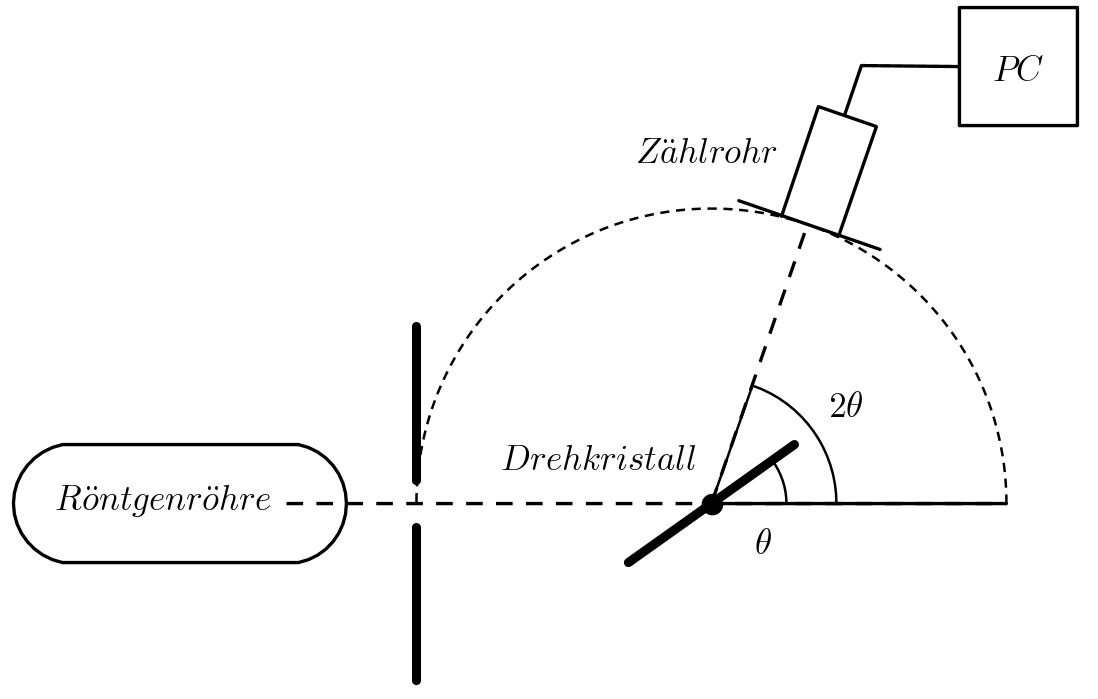
\includegraphics[width=0.8\textwidth] {pics/602f.png}
\centering
\caption{Schematischer Aufbau}
\label{Aufbau}
\end{figure}


Die Winkel des Einkristalls und des Zählrohrs sind beide voll automatisch über den Computer einstellbar. Ein Impulsratemeter
kann die vom Zählrohr erfassten Impulse verarbeiten. Aufgrund der Tatsache, dass die Emission von Röntgenquanten nicht
einheitlich ist und damit unregelmäßigen Schwankungen unterliegt, wird die Messgenauigkeit herabgesetzt. Hierzu wird die
Zeitkonstante des Impulsmeters mit dem PC auf 10 s gesetzt. Dies wiederum hat den Nachteil, dass rapide Zählratenänderungen
übergangen werden und damit beispielsweise die Absorbtionskanten nicht mehr wahrgenommen. Daher sind mehrere Durchführungen
mit verschiedenen Zeitkonstanten erforderlich, um die besten Messergebnisse zu erzielen. Da die beiden Winkel ein Verhältnis
von 2:1 haben, ist stets die Bragg-Reflexionsbedingung gegeben, womit die Strahlintensität in Abhängigkeit des Winkels
$\theta$ und damit die Energie nach \eqref{Bragg} aufgetragen werden kann. 

Das Emissionsspektrum wird ohne Befestigung einer Materialprobe in einem Winkelbereich für $7^\circ \le \theta \le 30^\circ$ ausgemessen.
Zur Aufnahme des Absorbtionsspektrums wird die Probe auf die Blende des Zählrohrs geschraubt und in einem Winkelbereich von
$9^\circ \le \theta \le 20^\circ$ erstellt.\\
Untersuchte Materialien sind: $_{32}$Germanium, $_{38}$Strontium, $_{79}$Gold, $_{83}$Wismut

\section{Auswertung}

\section{Diskussion}

% ========================================
%	Literaturverzeichnis
% ========================================
$_{32}$
%\bibliographystyle{plainnat}			% Bibliographie-Style auswählen
%\bibliography{BIBDATEI}			% Literaturverzeichnis
$_{32}$
% ========================================
%	Das Dokument endent
% ========================================

\end{document}
